\section{Results and Discussion}

\begin{description}

\begin{figure}
\centering
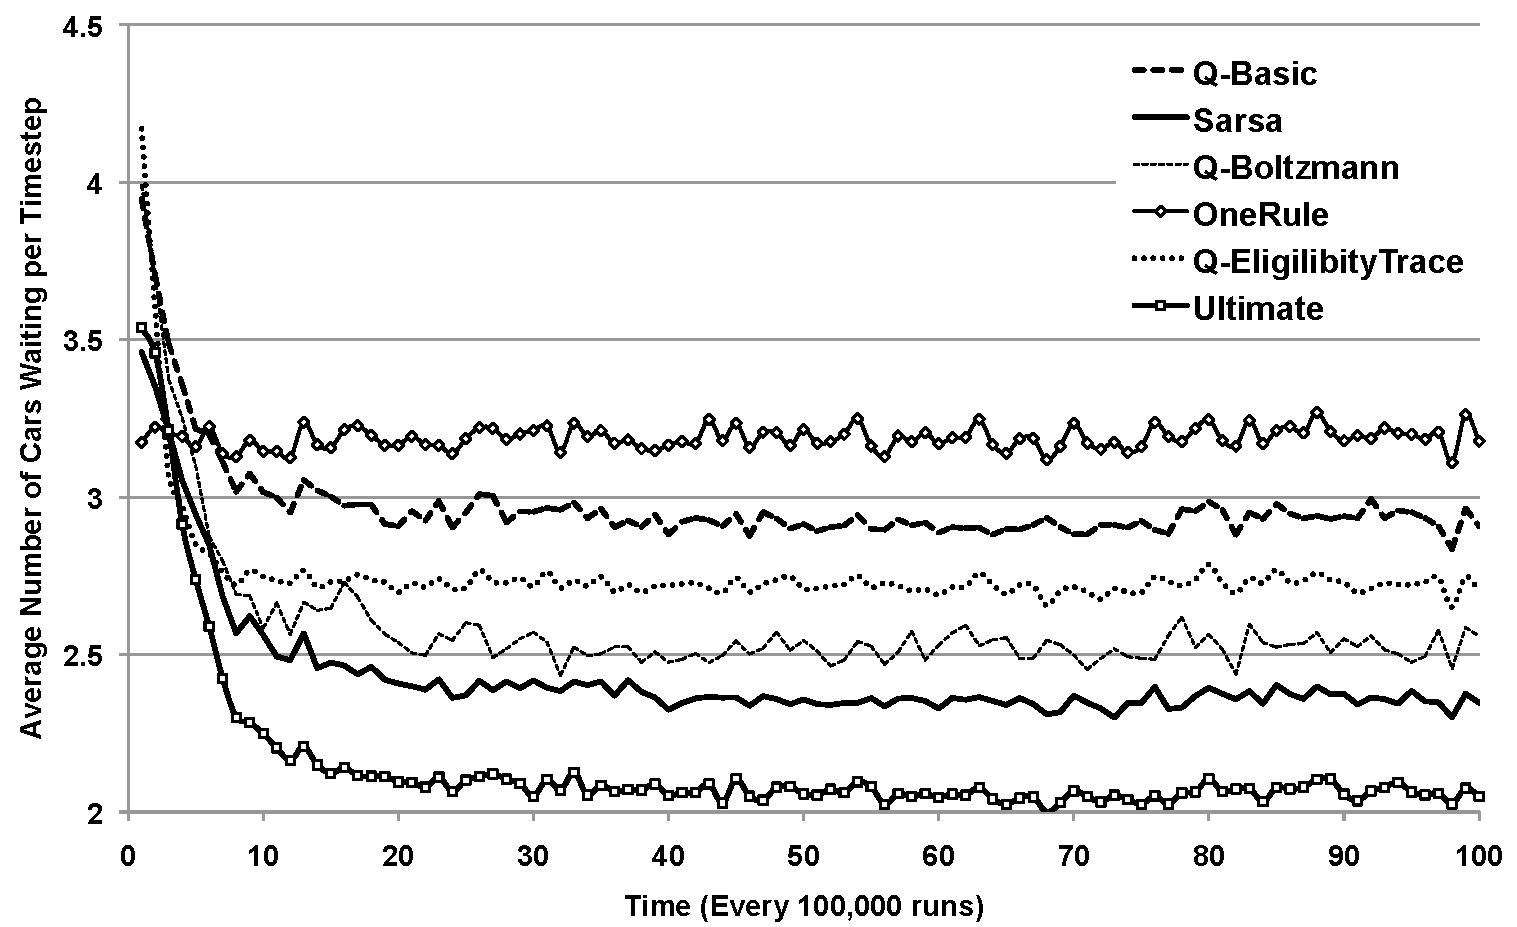
\includegraphics[width=0.45\textwidth]{algorithm}
\caption{Best Algorithm}\label{f:algorithm}
\end{figure}

\item[Fig.~\ref{f:algorithm}] To determine the best choice of algorithm we ran
an experiment using five configurations of algorithms and refinements whilst
keeping the state representation, learning rate, discount factor and traffic
intensity constant in accordance with the benchmark setup. We also ran the
benchmark setup labelled as Q-Basic. The best algorithm without refinements
running against the benchmark setup is the Sarsa algorithm converging to just
under 2.5 waiting cars per timestep. The Q-Learning algorithm's performance is
best when using Boltzmann's action selection policy and also benefits from the
use of an eligibility trace but is still beaten by the Sarsa algorithm.
 The Ultimate algorithm is a modified version of the Sarsa algorithm using an
 action selection
policy which chooses an action with probability $p$ from the Boltzmann
distribution rather than using the $\epsilon$-greedy strategy, and includes the
use of eligibility traces. The Ultimate algorithm delivers significantly better
performance than all other experiements after 1,000,000 timesteps and converges
with just above 2 cars waiting per timestep on average.

\begin{figure}
\centering
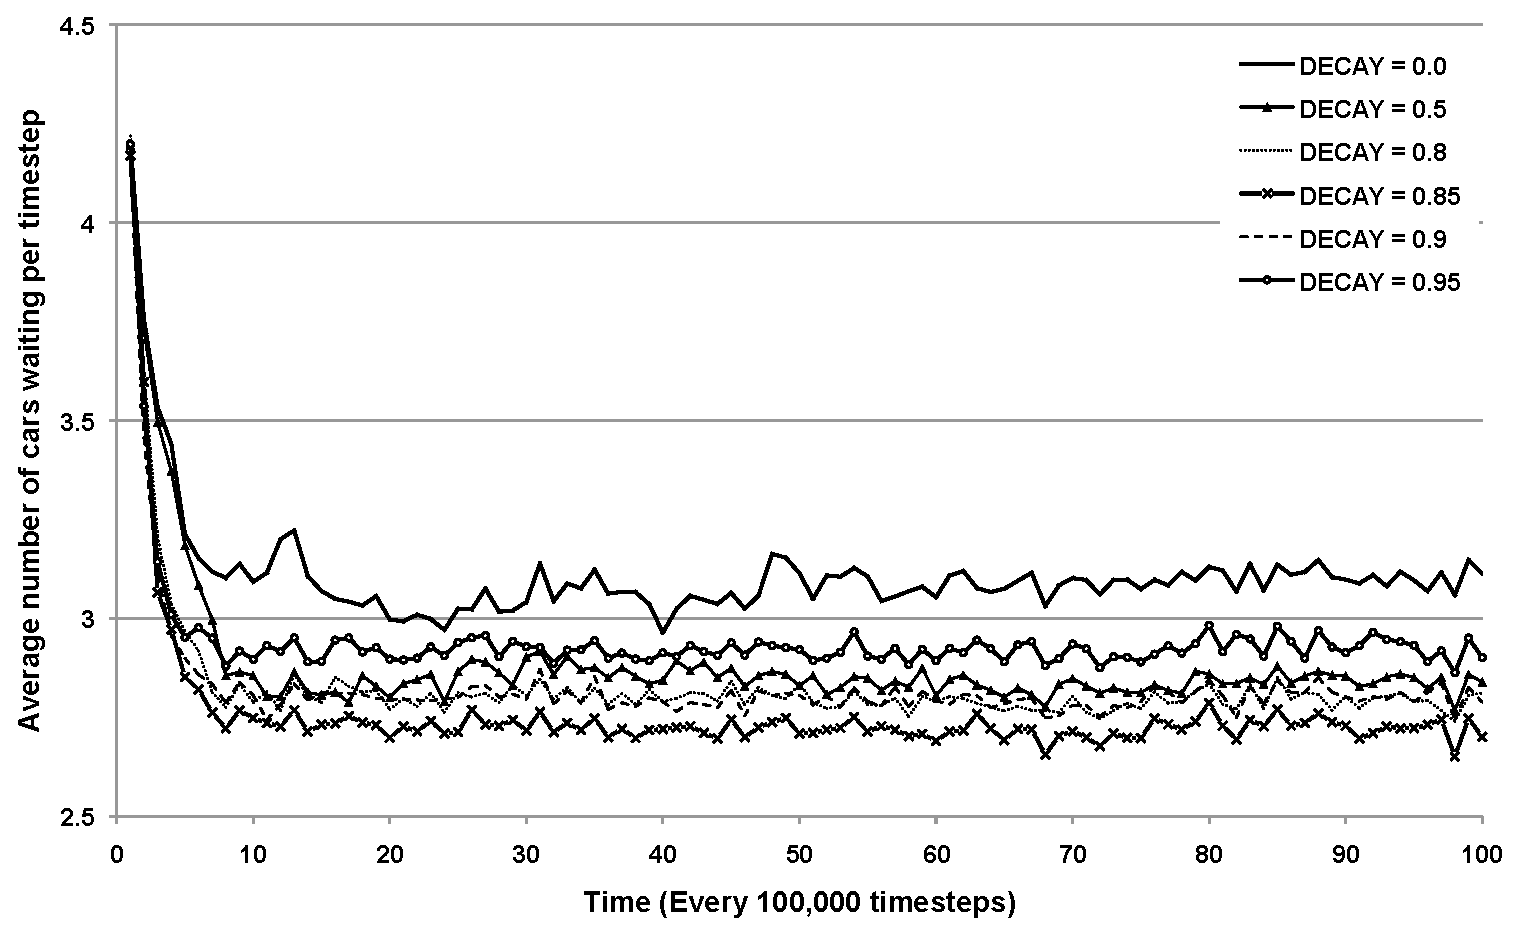
\includegraphics[width=0.45\textwidth]{eligibility}
\caption{Eligibility Trace}\label{f:eligibility}
\end{figure}

\item[Fig.~\ref{f:eligibility}] From varying the eligibility decay factor over
our benchmark setup, we observed the ideal decay to be set to 0.85 however it is
evident that this factor alone has little impact on the performance of the
overall algorithm.

\begin{figure}
\centering
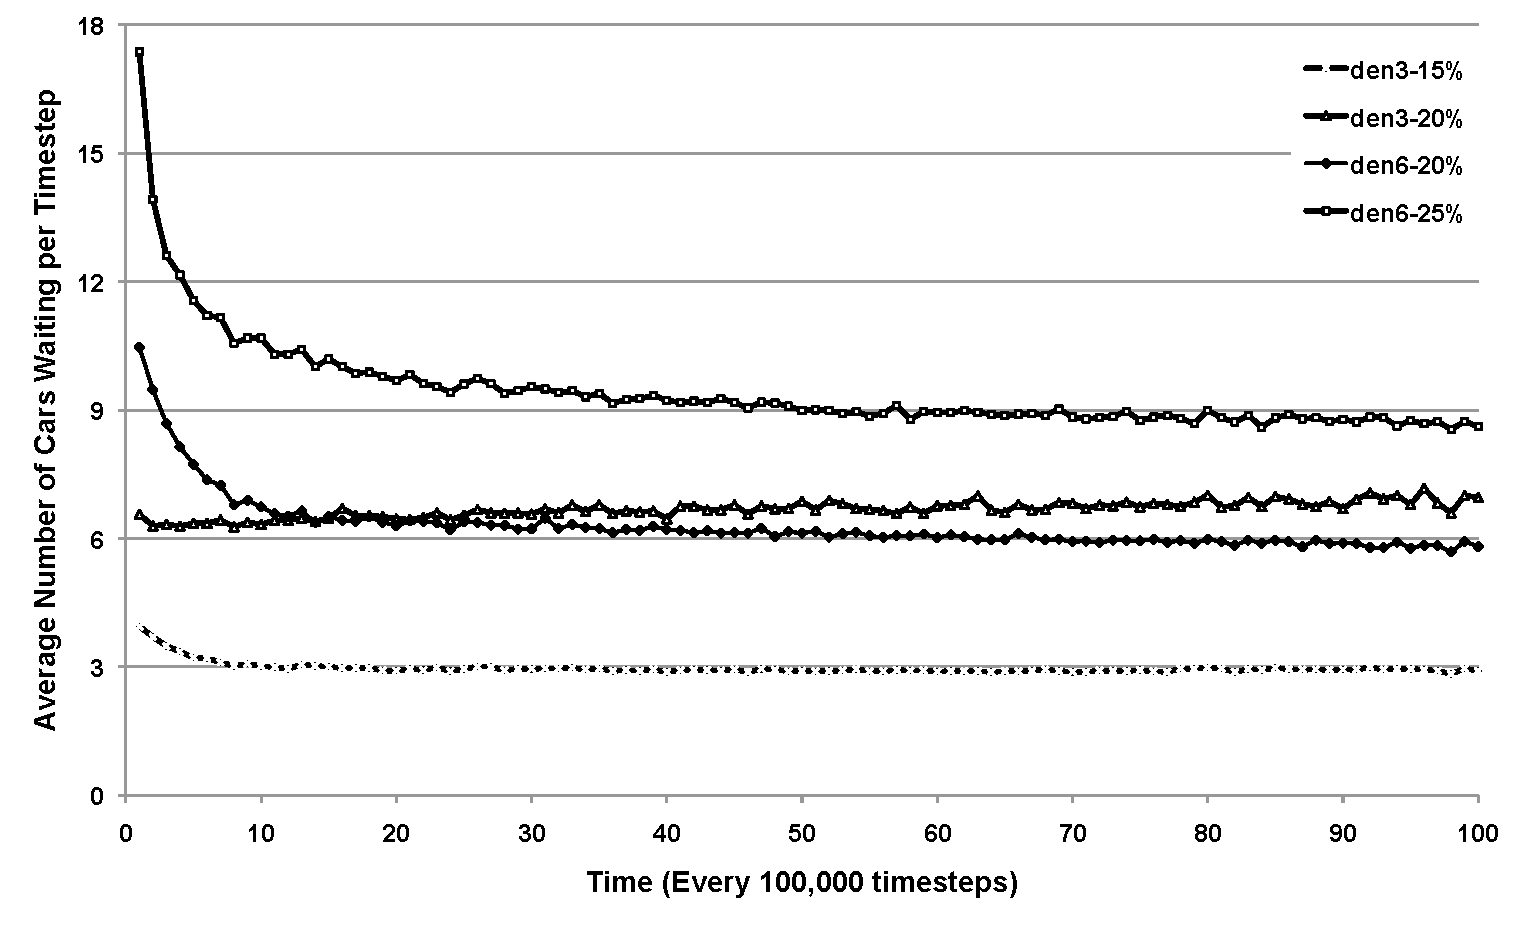
\includegraphics[width=0.45\textwidth]{intensity}
\caption{Varying Traffic Intensity}\label{f:intensity}
\end{figure}

\item[Fig.~\ref{f:intensity}] Perhaps unsurprisingly, as the traffic intensity
increases from 15\% to 25\%, we found more cars waiting for a green light with
an overall performance drop. Using Density\_3 and Density\_6 at 20\% traffic
intensity, we observed similar performance over 2,000,000 timesteps. However,
Density\_3 --- having a smaller state space --- starts to overfit the traffic
patterns whereas Density\_6 --- having a larger state space --- continues to
converge to optimal. Also, Density\_6 takes longer to converge relative to
Density\_3, most likely due to the larger state space.

\begin{figure}
\centering
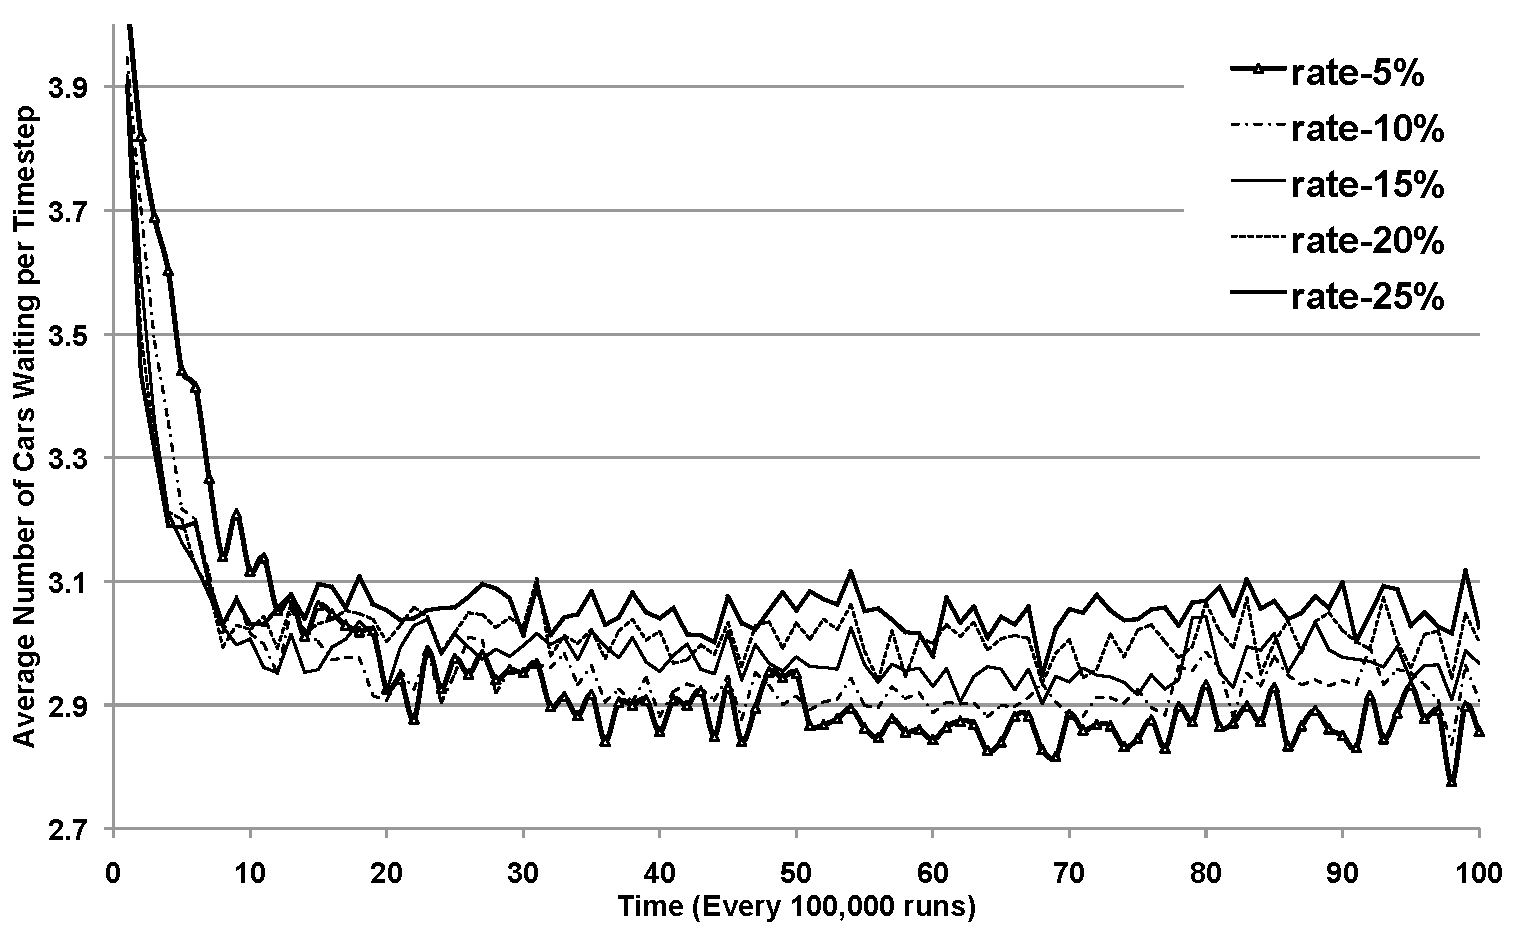
\includegraphics[width=0.45\textwidth]{learningRate}
\caption{Varying Learning Rate}\label{f:learningRate}
\end{figure}

\item[Fig.~\ref{f:learningRate}] In this experiement we vary the learning rate
from 5\% to 25\% using the benchmark setup. It was observed that the optimal
learning rates were between 5\% and 10\% evident after 2,000,000 timesteps.
However, up until 1,000,000 timesteps a learning rate of 5\% produces a
significantly higher number of waiting cars than learning rates above 10\%.
Given the small difference between the number of waiting cars between 5\% and
10\%, we would consider a learning rate of 10\% more optimal.

\begin{figure}
\centering
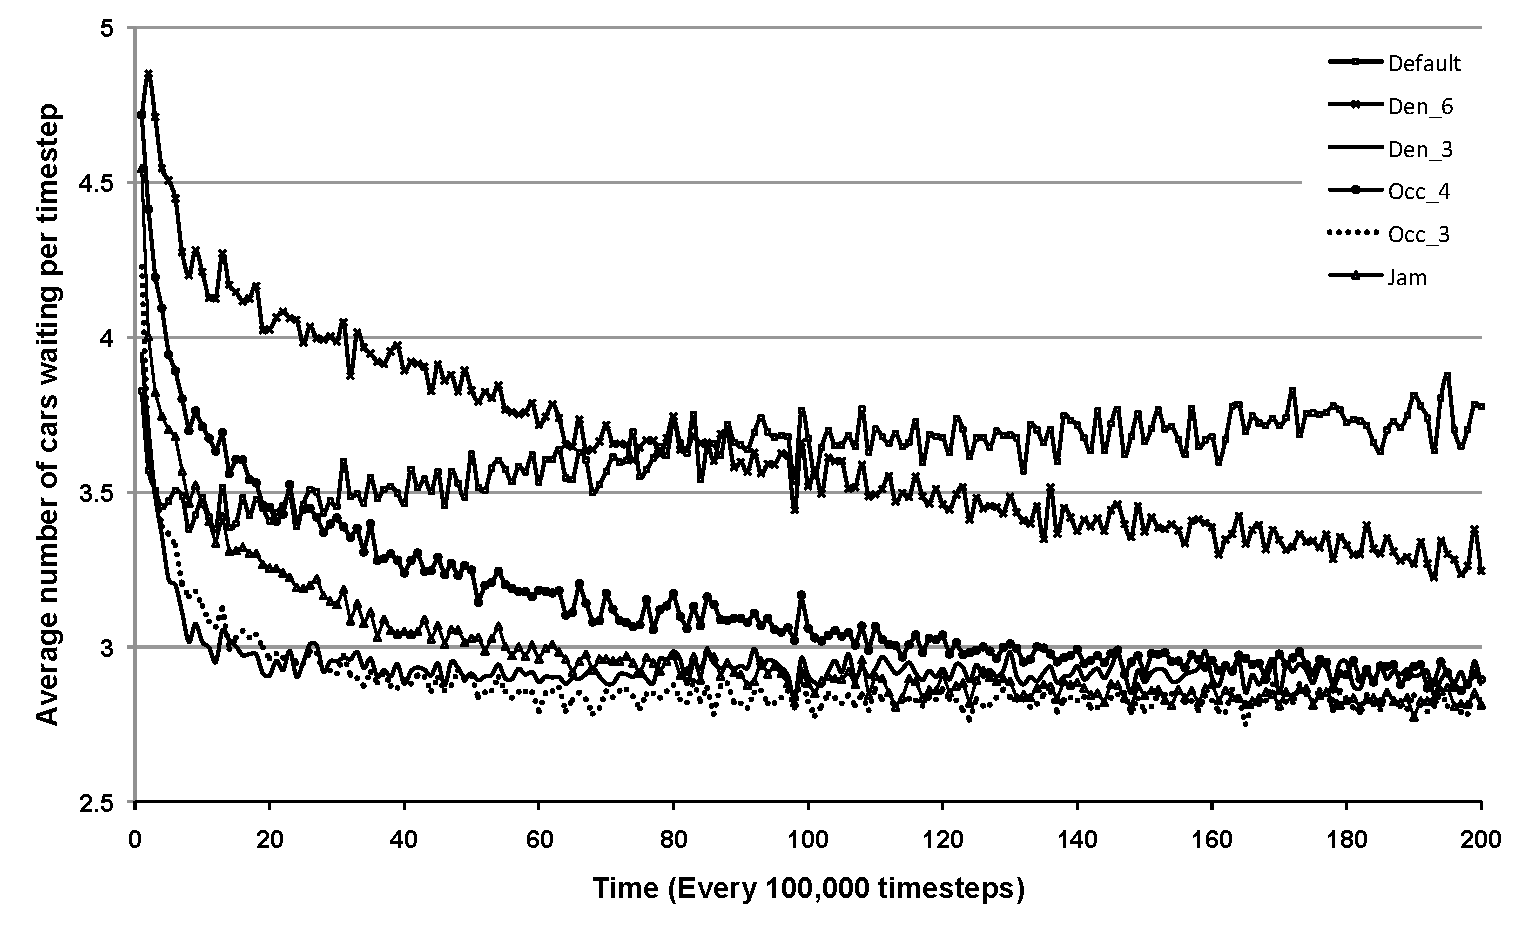
\includegraphics[width=0.45\textwidth]{states}
\caption{Varying State Representation}\label{f:states}
\end{figure}

\item[Fig.~\ref{f:states}]
This experiment uses the benchmark settings while varying the state space representation. The Default state produces the most sub-optimal performance after 2,000,000 timesteps. This representation provides quite a large state space but the type of information being conveyed is less useful than other representations as we only have information about one car on each road at any one time, giving no indication of how busy the traffic is which is the ultimate cause of accumulation of negative rewards. This is in contrast to the Occupancy, Density and JamNess spaces which provide a much better indication of how busy a road is in this sense. This is reflected in our experiment by the convergence of this group after 2,000,000 timesteps to between 2.7 to 3.0 average waiting cars. An interesting observation is the large difference between Density\_6 and Density\_3 spaces with Density\_3 converging with the other best performing representations while Density\_6 lags behind the group while narrowing in over the duration of the experiment. Occ\_3 also performs better than Occ\_4 initially. This is to be expected as it is logical that large state spaces will be slower to converge than smaller state spaces.

\begin{figure}
\centering
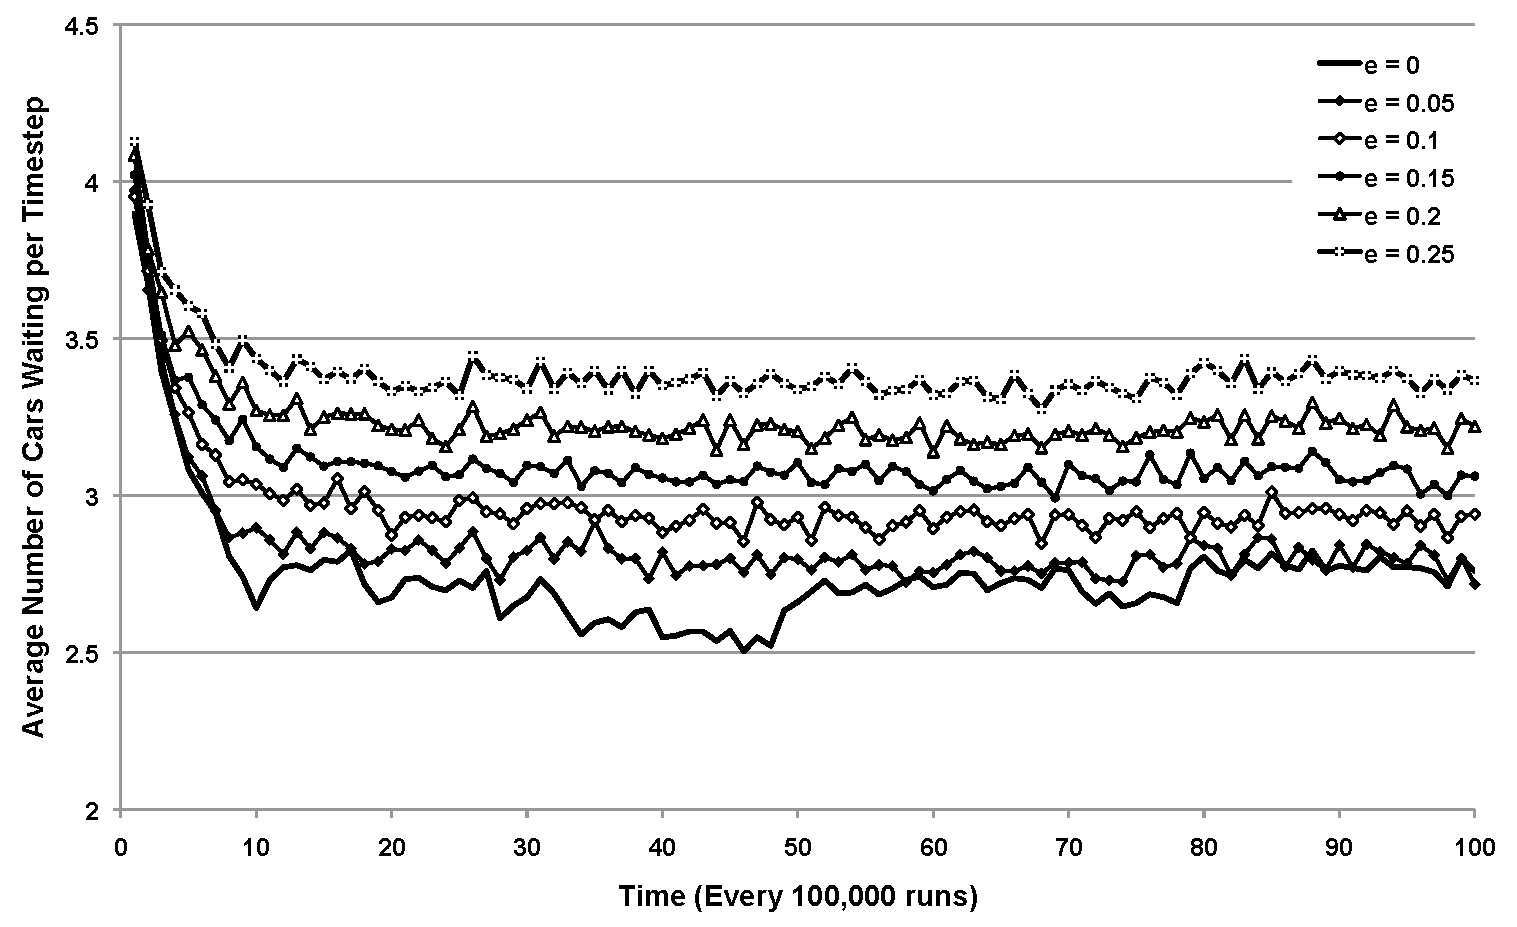
\includegraphics[width=0.45\textwidth]{epsilon}
\caption{Varying the $\epsilon $ value}\label{f:epsilon}
\end{figure}

\item[Fig.~\ref{f:epsilon}]
This experiment uses the benchmark settings except for the $\epsilon$
value (`e' in the figure) which is different in each run. For example $e = 0.25$ means
the QLearningBasic algorithm will explore 25\% of the time.
Note the $\epsilon$ is not discounted over time.
Better results are achieved with $\epsilon$ values near 0 but not 0,
suggesting that exploratory actions
that are not optimal are adding to the number of cars waiting; so
the less exploratory actions taken the better. However, some exploration
is required since $\epsilon =0$ shows that overfitting occurs after
about 4,600,000 timesteps. This overfitting is most likely due to
the algorithm finding the optimal action-value function for the traffic
pattern in the first 4.6 million timesteps, but the traffic patterns
in the following timesteps are different and the optimal policy is
no longer the most optimal.

\begin{figure}
\centering
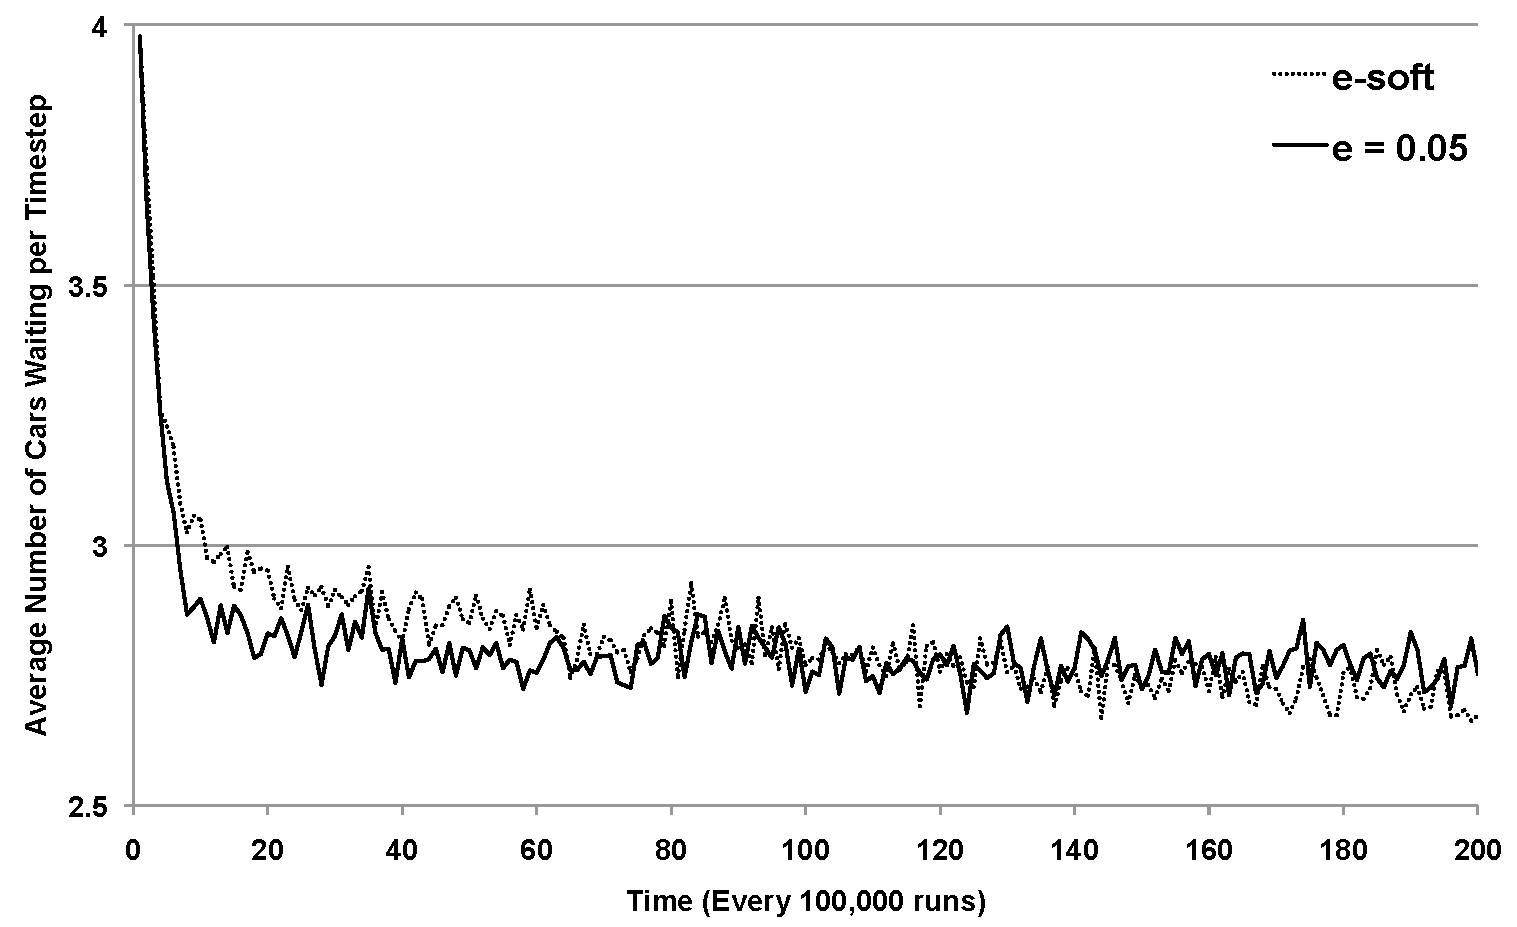
\includegraphics[width=0.45\textwidth]{e-soft}
\caption{Discounting $\epsilon$}\label{f:e-soft}
\end{figure}

\item[Fig.~\ref{f:e-soft}]
This figure shows the $\epsilon = 0.05$ result with a discounted
$\epsilon$ run. The discounted $\epsilon$ run uses the benchmark
settings (i.e. $\epsilon = 0.1$ initially) and discounting the
$\epsilon$ by 0.9999999 per timestep (that's seven 9s). The result shows
that a fixed $\epsilon$ stablises after about 4,300,000 timesteps
without further improvement; but the $\epsilon$-discounted algorithm
converges to the optimal as time progresses. This matches with what Sutton
\cite{sutton_rl_1998} says about Sarsa converges with probability
1 to an optimal policy only if the policy converges in the
limit to the greedy policy (i.e. $\epsilon$ tends to 0 in the limit);
although this is QLearningBasic algorithm and not Sarsa.

\begin{figure}
\centering
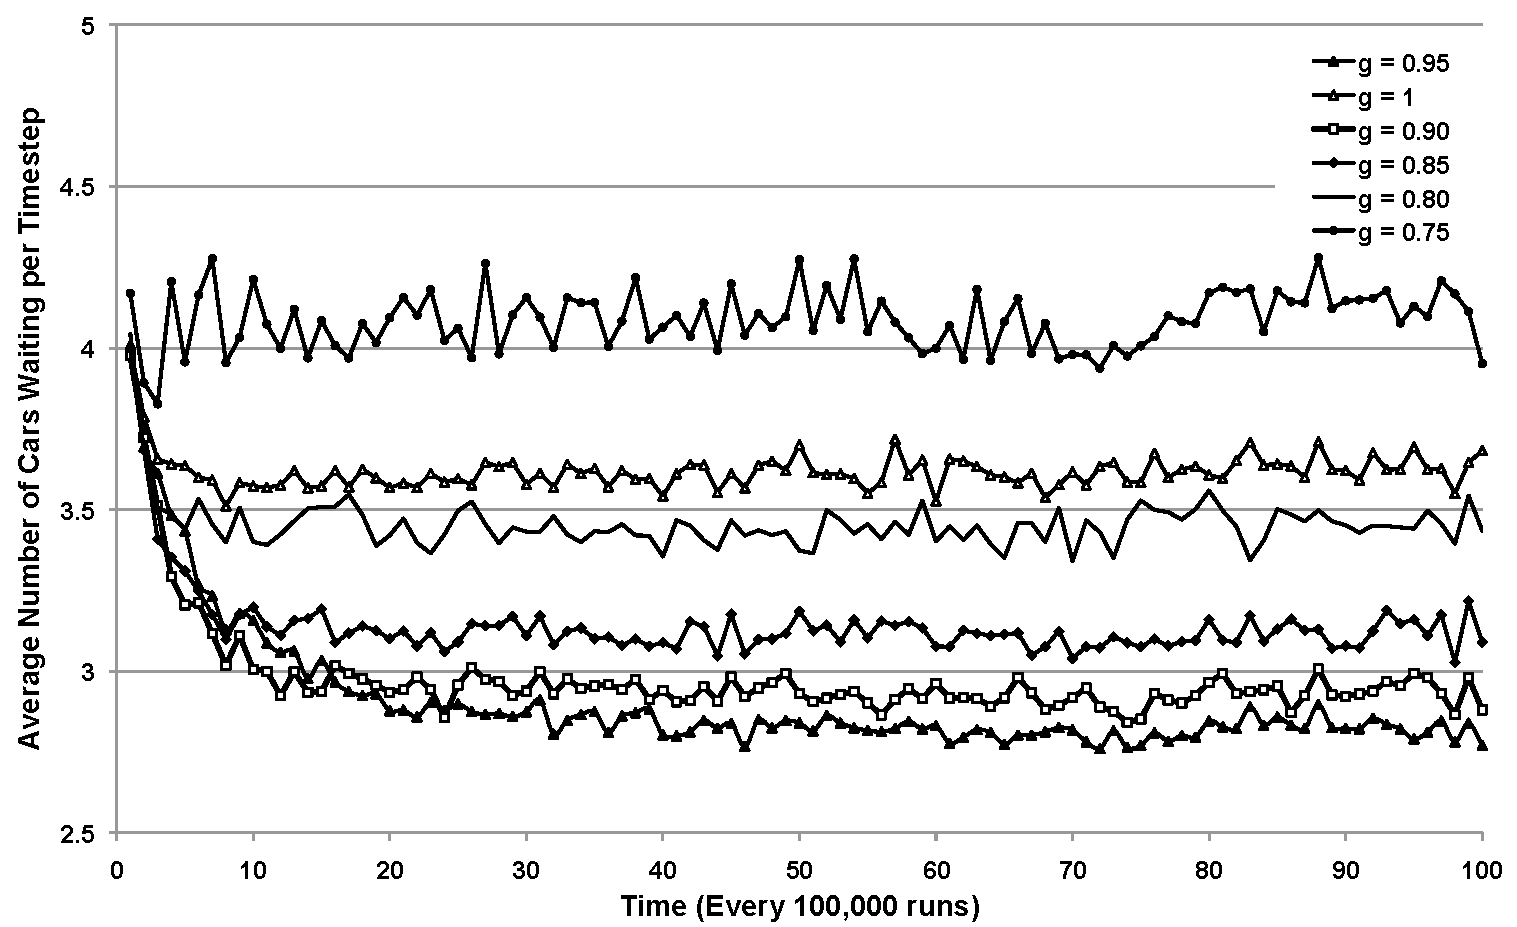
\includegraphics[width=0.45\textwidth]{discountFactor}
\caption{Varying the discount factor $\gamma$}\label{f:discountFactor}
\end{figure}

\item[Fig.~\ref{f:discountFactor}]
This experiment uses the benchmark settings except for the $\gamma$
discount factor (`g' in the figure) which is different in each run.
The results suggest the best discount factor to use is 0.95. As
$\gamma$ decreases from 0.95, the results gets progressively worse.
Values larger than 0.95 should also get worse, although only one run with $\gamma = 1$.

\end{description}

